%%%%%%%%%%%% Attribution %%%%%%%%%%%%
% This template was created by 
% Chuck F. Rocca at WCSU and may be
% copied and used freely for 
% non-commercial purposes.
% 10-17-2021
%%%%%%%%%%%%%%%%%%%%%%%%%%%%%%%%%%%%%

%%%%%%% Start Document Header %%%%%%%
% In creating a new document
% copy and paste the header 
% as is.
%%%%%%%%%%%%%%%%%%%%%%%%%%%%%%%%%%%%%

\documentclass[12pt]{article}

%%%% Header Information %%%%
    %%% Document Settings %%%%
    \usepackage[utf8]{inputenc}
    \usepackage[
        twoside,
        top=1in,
        bottom=0.75in,
        inner=0.5in,
        outer=0.5in
    ]{geometry}
    \pagestyle{myheadings}

%%%% Additional Commands to Load %%%%
    \usepackage{tcolorbox}
    \tcbuselibrary{skins}
    \usepackage{minted}
    \usepackage{color}
    \usepackage{tikz}
    \usetikzlibrary{calc}
    \usepackage{tabularx,colortbl}
    \usepackage{amsfonts,amsmath,amssymb}
    \usepackage{titling}
    \usepackage{mathrsfs}
    \usepackage{calc}
    \usepackage{xepersian}

%%%% Commands to Define Homework Boxes %%%%
%%%% Box Definition %%%%
    \newtcolorbox{prob}[1]{
    % Set box style
        sidebyside,
        sidebyside align=bottom,
    % Dimensions and layout
        width=\textwidth,
        toptitle=2.5pt,
        bottomtitle=2.5pt,
        righthand width=0\textwidth,
    % Coloring
        colbacktitle=gray!30,
        coltitle=black,
        colback=white,
        colframe=white,
    % Title formatting
        title={
            #1 \hfill نمره:\phantom{WWWW}
        },
        fonttitle=\large\bfseries
    }

%%%% Environment Definition %%%%
    \newenvironment{problem}[1]{
        \begin{prob}{#1}
    }
    {
        \tcblower
        \centering
        \vspace{\baselineskip}
        \end{prob}
    }



%%%% Document Information %%%%
    \title{تکلیف سری سوم درس کنترل دیجیتال}
    \date{نیسمال دوم 1402-1403}
    \author{استاد درس : دکتر طالبی}
    \usepackage{amsmath}

%%%%%%% End Document Header %%%%%%%


%%%% Begin Document %%%%
% note that the document starts with
% \begin{document} and ends with
% \end{document}
%%%%%%%%%%%%%%%%%%%%%%%%
\settextfont{BNAZANIN.TTF}

\begin{document}

%%%% Format Running Header %%%%%
\markboth{\theauthor}{\thetitle}

%%%% Insert the Title Information %%%
% \maketitle


%%%% General Description of the Document %%%%
\begin{figure}[htbp]
    \centering
    
\includegraphics[width=\linewidth]{Header.png}
    % \caption{Caption}
    % \label{fig:enter-label}
\end{figure}


%%%% Introduction to the General Template %%%%
\section{بخش اجباری}

    \begin{problem}{سوال اول}
    (تبدیل ستاره\lr{SFG}) در سیستم نمونه برداری شده شکل زیر تنها با استفاده از روش مدل گذر سیگنال ، 
    $C(z)$
    و
    $C(s)$
    را بدست آورید.

    \end{problem}
    
    \begin{figure}
    	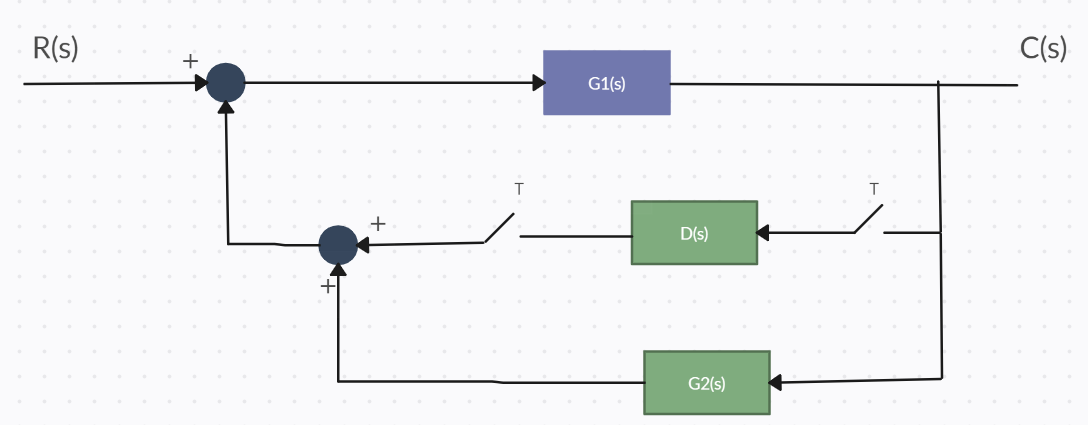
\includegraphics[width=\linewidth]{Resources/3.png}
    	\caption{شکل سوال اول}
    \end{figure}
    
    \begin{problem}{سوال دوم}
  (گسسته سازی (انتگرال عددی)) تابع یک سیستم \lr{lag} می باشد که برای افزایش 10 برابری 
  $K_v$
  طراحی شده شده از و میزان پیشفازی در 
  $\omega_1 = 3 rad$
  قابل صرف نظر دارد.
  
  این تابع تبدیل را با دو روش 
  \lr{Forward}
  و
  \lr{Backward}
  گسسته سازی کنید مقدار پسفازی را در 
  $\omega_1 = 3 , T = 0.25s$
  بدست آورید و با مقدار اصلی مقایسه کنید.
  
  \centering
 $H(s) = 10\frac{10s + 1}{100s + 1}$
    \end{problem}
    
    \begin{problem}{سوال سوم}
    	(گسسته سازی (انتگرال عددی))
سوال قبل را به روش 
\lr{Tustin with prewarping}
و فرکانس 
\lr{Prewarping}
برابر 
$\omega_{pw} = 3 rad/s$
بدست آوردید.
نتایج را با سوال قبل مقایسه کنید.
    \end{problem}
    
    
    \begin{problem}{سوال چهارم}
    	(گسسته سازی (تطبیق صفر و قطب)) سوال دوم را به روش تطبیق قطب و صفر حل کنید و با نتایح سوالات دوم و سوم مقایسه کنید
    	
    	
    \end{problem}
    
    \begin{problem}{سوال پنجم}
    	(گسسته سازی (فضای حالت)) معادل گسسته سیستم با معادلات حالت زیر را پیدا کنید.
    	از نگهدار مرتبه صفر استفاده کنید.
    	
    	    	\centering
    	$
    	\dot{x}(t)=Ax(t)+Be(t) 
    	$
    	
    	$
    	y(t)=Cx(t)+D 
    	$
    	
    	$
    		 A=\left( \begin{matrix}
    			0 & 1 \\  
    			-1 & -1 \\ 
    		\end{matrix} \right),B=\left( \begin{matrix}
    			0 \\
    			1  
    		\end{matrix} \right)  
    		 C=\left( \begin{matrix}
    			1 & 0  
    		\end{matrix} \right) 
    	$
    \end{problem}
    
    \begin{problem}{سوال ششم}
    	(گسسته سازی (فضای حالت)) معادله زیر شکل کلی فضای حالت را نشان می‌دهد. با استفاده از آن شکل کلی فضای حالت گسسته سازی شده به روش دو خطی (\lr{bilinear}) را بدست آورید.
    
    	\centering
$
    		 \dot{x}(t)=Ax(t)+Be(t) 
$

$
    		 y(t)=Cx(t)+D 
$
    	
	
	
	\end{problem}    
    
\section{بخش امیتازی}
    \begin{problem}{سوال هفتم}
	(مدارات تبدیل آنالوگ و دیجیتال)(\lr{R-2R Ladder})
	در مدار نشان داده شده در شکل 
	$R = R_f = 10K\Omega$
	و
	$V_R = 5V$
	عدد دیجیتال توسط متغیر های $S_0$ ، $S_1$ ، $S_2$ و $S_3$ نشان داده شده است که در آن 
	$S_3$
	نقش پر ارزش ترین بیت را دارد. ولتاژی که در نقطه 
	$A_k$
	قرار دارد همان 
	$V_R$
	است. هر گاه 
	$S_k = 1$
	باشد و در غیر این صورت $0$ ولت می باشد. اگر 
	$S_1 = 1$
	باشد و سایر بیت ها برابر صفر باشند. مطلوب است مقدار $V_0$
	
	\end{problem}   
	\begin{figure}
		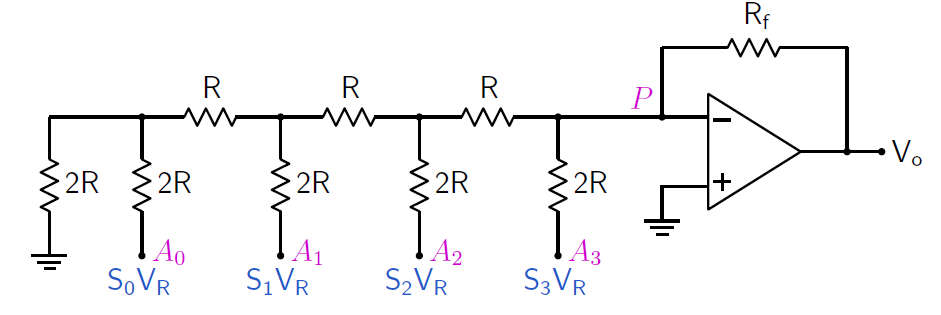
\includegraphics[width=\linewidth]{Resources/1.png}
		\caption{شکل سوال هفتم}
	\end{figure}
    \begin{problem}{سوال هشتم}
	(مدارات تبدیل آنالوگ و دیجیتال)(\lr{SAR}) ولتاژ ورودي در یک \lr{ADC} هشت بیتی ار نوع \lr{SAR} برابر $13.478$ ولت می باشد. ولتاژ رفرنس \lr{ADC}
	نیز 20 ولت م یباشد. با استفاده از الگوریتم تبدیل عدد آنالوگ به دیجیتال در این نوع از \lr{ADC} ،
	مقدار عدد دیجیتال را بدست آورید.
	
	
	
	\end{problem}
	\begin{figure}
		\centering
		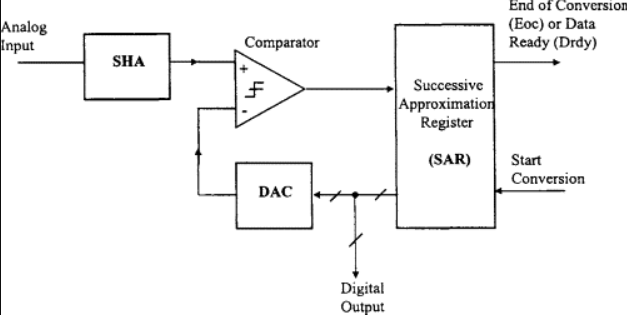
\includegraphics[scale=0.7]{Resources/2.png}
		\caption{شکل سوال هشتم}
	\end{figure}

\end{document}
